% !TEX root = ../main.tex
\documentclass[../main.tex]{subfiles}

\begin{document}
\section{Gleichstromverstärkung eines NPN-Transistors}

\subsection{Ziel}

Die Gleichstromverstärkung des ausgewählten NPN-Transistors \textit{BC548B} wird durch Messen des Kollektor- und Basisstroms hergeleitet und wird mit den Informationen vom Datenblatt verglichen. 


\subsection{Berechnungen}

Das Gleichstromverstärkungsverhalten ist in den Datenblätter entweder als $B$ oder als $h_{FE}$ beschrieben und gibt den Verstärkungsfaktor von $I_B$ zu $I_C$ an. Dieser Faktor basiert auf dem Verhältnis zwischen den beiden Strömen, welches in Gleichung \ref{equ:bjt_amplification} aufgezeigt wird.

\begin{equation}
    B = \frac{I_C}{I_B}
    \label{equ:bjt_amplification}
\end{equation}

Die maximale Verlustleistung ist als $P_{tot} = \SI{500}{\milli\watt}$ im Datenblatt des \textit{BC548B} angegeben. Somit errechnet sich über Gleichung \ref{equ:bjt_maxUce} eine maximale \textit{Collector-Emitter-Spannung} von 5V, wenn mit dem maximalen Kollektor-Strom von $\SI{100}{\milli\ampere}$. Die Messung wird mit diesen $U_{CE} = \SI{5}{\volt}$ und einer Strombegrenzung von $\SI{80}{\milli\ampere}$ durchgeführt, so bewegt sich der Arbeitspunkt immer in einem sicheren Rahmen.

\begin{equation}
    U_{CE_{max}} = \frac{P_V}{I_{C_{max}}} = \frac{\SI{500}{\milli\watt}}{\SI{100}{\milli\ampere}} = \SI{5}{\volt}
    \label{equ:bjt_maxUce}
\end{equation}

Mit dem maximalen Kollektorstrom definiert, wird der Basis-Strom mit dem Verstärkungsfaktor $h_{FE} = 200$, welcher vom Datenblatt des \textit{BC548B}s entnommen wurde, berechnet.

\begin{equation}
    I_B = \frac{I_C}{h_{FE}} = \frac{I_C}{200} = \SI{400}{\micro\ampere}
\end{equation}

Der \textit{Basis-Strom} soll mit einer \textit{Controll-Voltage} ($U_{CTRL}$ oder $U_{PS1}$) von bis zu $U_{CTRL_{max}} = \SI{10}{\volt}$ zwischen $I_B = \SI{0}{\micro\ampere}$ und $\SI{400}{\micro\ampere}$ moduliert werden können. Somit ergibt sich über Gleichung \ref{equ:bjt_Rv} einen Vorwiderstand von $\SI{22}{\kilo\ohm}$.

\begin{equation}
    R_{V} = \frac{U_{CTRL} - U_{BE}}{I_{B}} = \frac{\SI{10}{\volt} - \SI{0.7}{\volt}}{\SI{400}{\micro\ampere}} = \SI{23.3}{\kilo\ohm} \Rightarrow \textrm{E12-Reihe } R_{V} = \SI{22}{\kilo\ohm}
    \label{equ:bjt_Rv}
\end{equation}

\subsection{Messschaltung}

\begin{figure}[h]
    \centering
    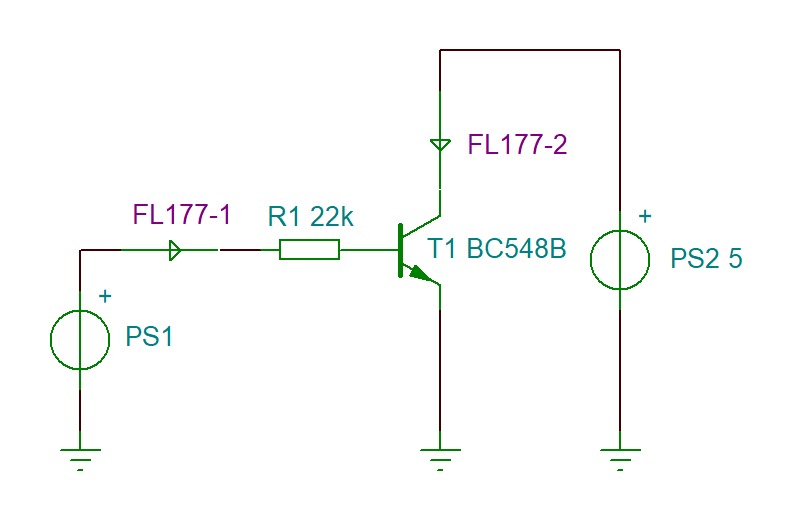
\includegraphics[scale=0.35]{assets/task1_DC_amplification/messschaltung_task1.PNG}
    \caption{Gleichstromverstärkung}
    \label{fig:circuit_dc_amplification}
\end{figure}

\subsection{Resultate}

\begin{table}[h]
\renewcommand{\arraystretch}{1.3}
\centering
\begin{tabular}{rrrrr}
\multicolumn{1}{c}{\textbf{$U_{PS1}$}} & \multicolumn{1}{c}{\textbf{$I_B$}} & \multicolumn{1}{c}{\textbf{$I_C$}} & \multicolumn{1}{c}{\textbf{$B$}} & \multicolumn{1}{c}{\textbf{$P_V$}} \\
\multicolumn{1}{c}{[$\si{\volt}$]} & \multicolumn{1}{c}{[$\si{\ampere}$]} & \multicolumn{1}{c}{[$\si{\ampere}$]} & \multicolumn{1}{c}{${I_C}/{I_B}$} & \multicolumn{1}{c}{[$\si{\watt}$]} \\ \hline
0.0 & 0.0E+0 & 0.0E+0 & \multicolumn{1}{c}{-} & 0.0E+0 \\
1.0 & 0.02E-3 & 4.7E-3 & 235.0 & 23.5E-3 \\
2.0 & 0.06E-3 & 18.0E-3 & 300.0 & 90.0E-3 \\
3.0 & 0.11E-3 & 29.8E-3 & 270.9 & 149.0E-3 \\
4.0 & 0.15E-3 & 38.2E-3 & 254.5 & 190.9E-3 \\
5.0 & 0.20E-3 & 42.8E-3 & 214.0 & 214.0E-3 \\
6.0 & 0.24E-3 & 46.4E-3 & 193.3 & 232.0E-3 \\
7.0 & 0.30E-3 & 49.5E-3 & 165.0 & 247.5E-3 \\
8.0 & 0.33E-3 & 52.0E-3 & 157.6 & 260.0E-3 \\
9.0 & 0.38E-3 & 54.4E-3 & 143.2 & 272.0E-3 \\
10.0 & 0.42E-3 & 56.6E-3 & 134.8 & 283.0E-3                          
\end{tabular}
\caption{Messresultate}
\end{table}

\begin{figure}[H]
    \centering
    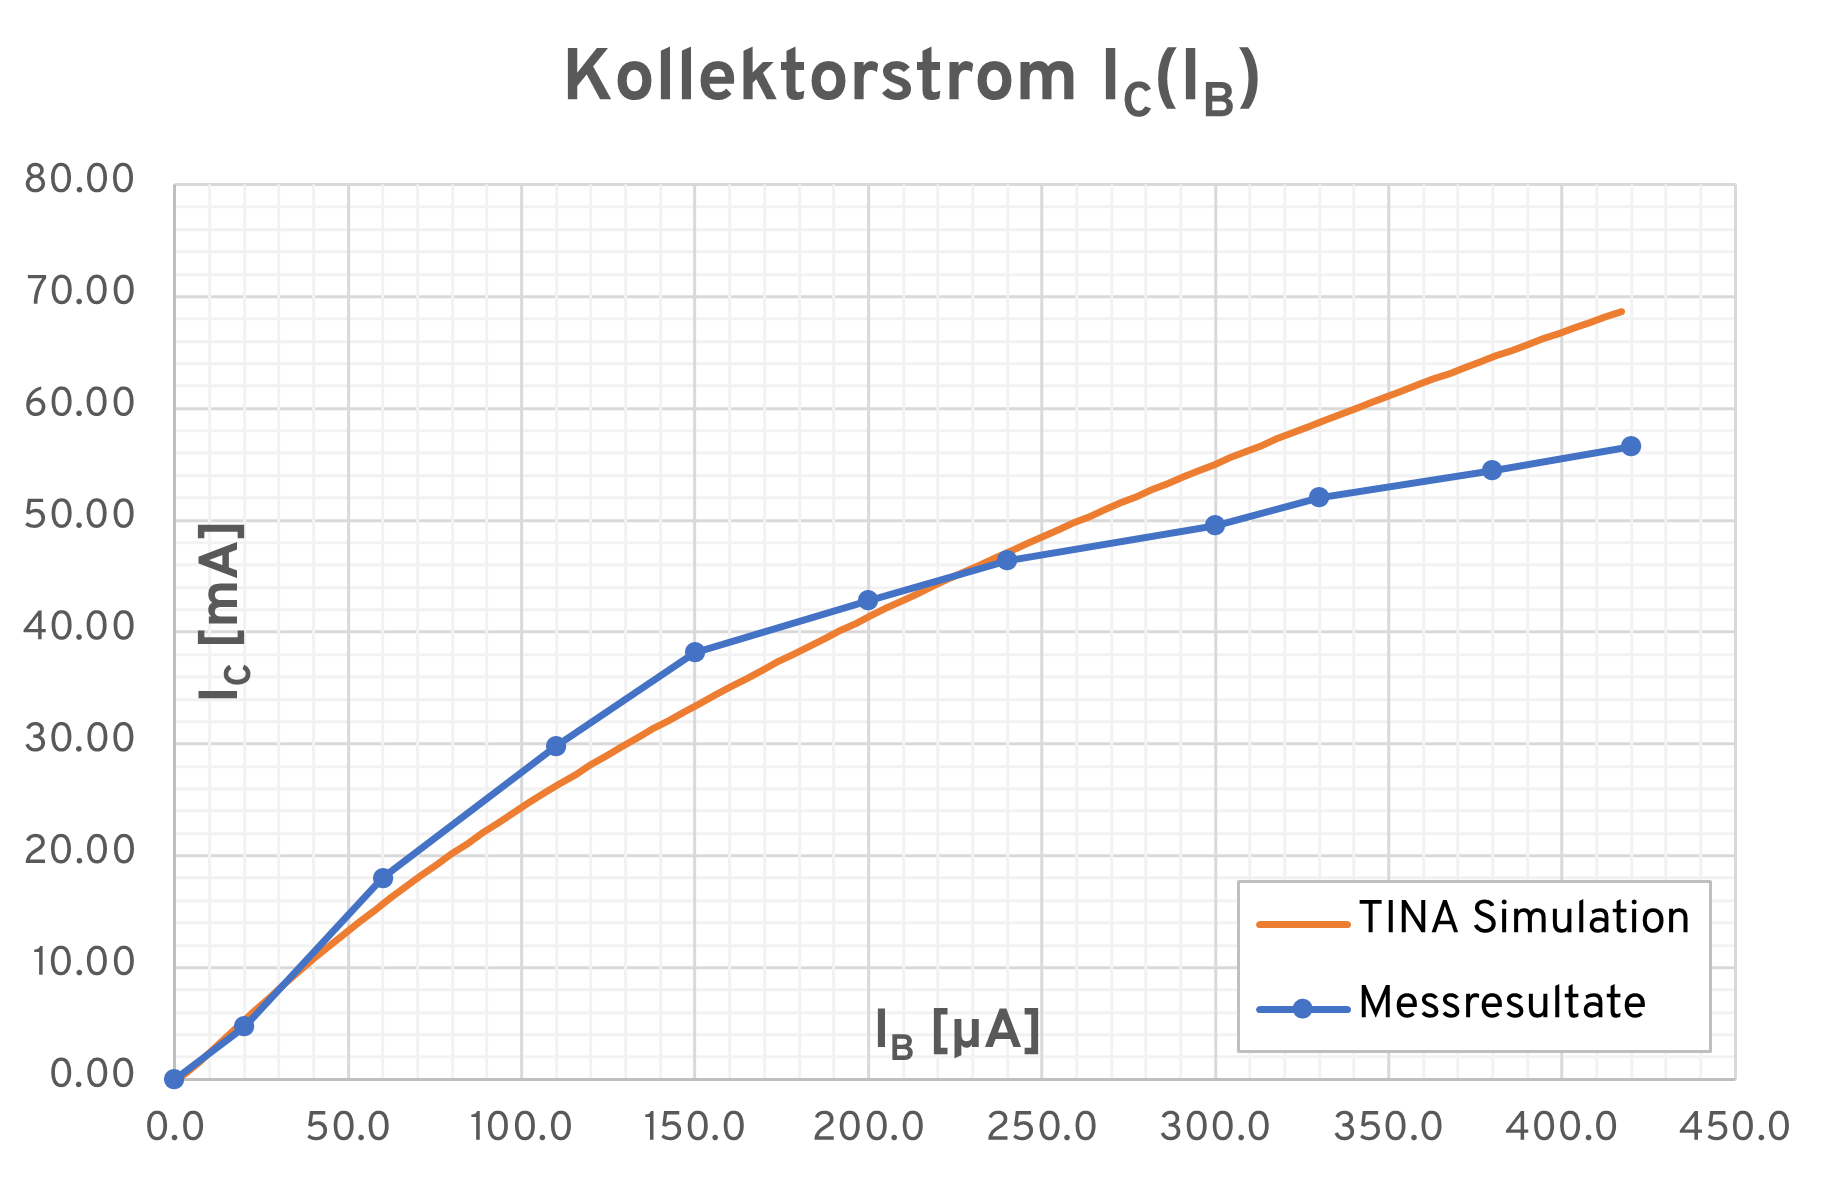
\includegraphics[scale=0.8]{assets/task1_DC_amplification/task1_IC_IB.png}
    \caption{$I_C(I_B)$-Diagramm mit Realwerten und TINA-Werten}
    \label{fig:diagram_results_IC_IB}
\end{figure}

\begin{figure}[H]
    \centering
    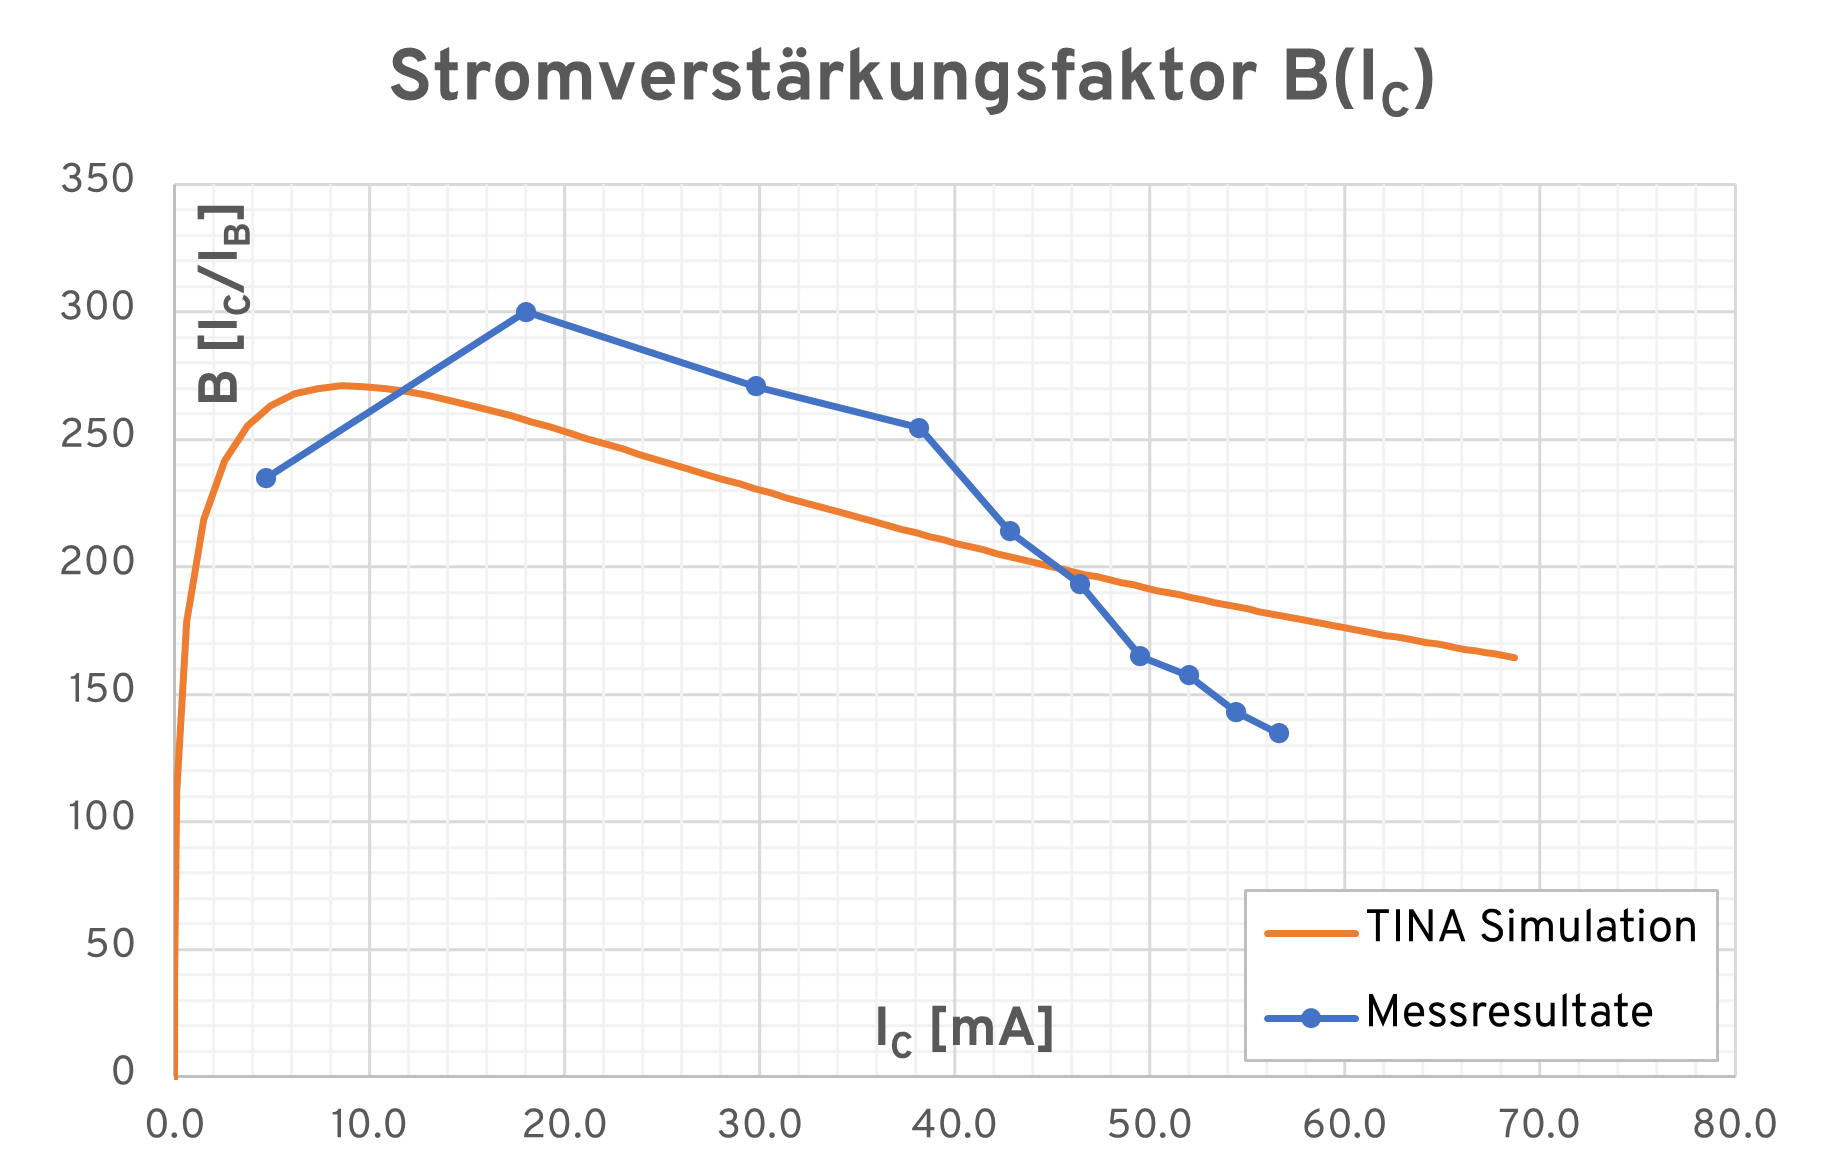
\includegraphics[scale=0.8]{assets/task1_DC_amplification/task1_B_IC.png}
    \caption{$B(I_C)$-Diagramm mit Realwerten und TINA-Werten}
    \label{fig:diagram_results_IC_B}
\end{figure}
\newpage
\subsection{Schlussfolgerung}

Die gemessenen Werte weisen einen ähnlichen Verlauf auf, wie die der TINA-Simulation. Im Vergleich zwischen der $B(I_C)$-Kurve (Abbildung \ref{fig:diagram_results_IC_B}) und der $h_{FE}(I_C)$-Kurve aus dem Datenblatt (Abbildung \ref{fig:datasheet_BC548B_IC_BFE}), scheint die Kurve des Datenblatts einen idealen Verstärkungsfaktor von $200$ bei $\SI{0}{\ampere}$ bis $\approx \SI{40}{\milli\ampere}$ anzugeben. Dies entspricht nicht mit den real Resultaten, wobei die realen weitere Einflüsse besassen, wie zum Beispiel den Widerstand der Steckbretter.

\begin{figure}[H]
    \centering
    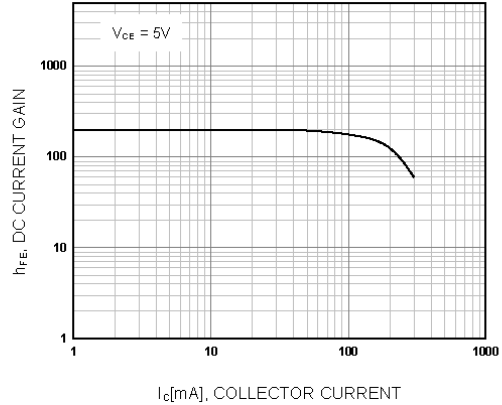
\includegraphics[scale=0.7]{assets/task1_DC_amplification/datasheet_BC548B_IC_HFE.png}
    \caption{Datenblattausschnitt vom $h_{FE}(I_C)$-Diagramm des \textit{BC548B}s}
    \label{fig:datasheet_BC548B_IC_BFE}
\end{figure}

Die Resultate der Abbildung \ref{fig:diagram_results_IC_IB} zeigen einen Verlauf auf, welche leicht einem linearen Verlauf ähnelt, wobei die Messresultate ab $I_B  \approx\SI{225}{\micro\ampere}$ an Steigung verliert. Wenn ein kleiner Bereich von $I_B$ verwendet wird, kann $I_C$ fast proportional/linear verstärkt werden. Aber sobald ein grösserer Bereich verwendet wird, wird $I_C$ stark verzerrt.

\end{document}